\begin{frame}{Construction of 1D Featureless Insulators}
\vskip-1.5cm		
\begin{columns}[T]
	\begin{column}[T]{.5\textwidth}
		\begin{block}{Classical Insulators}
			\vskip0.55cm
			\only<1, 2>{
			\begin{figure}
				
\includegraphics[width=\linewidth] {diagrams/trivial_chain.pdf}
				\caption{1D Trivial Chain}
			\end{figure}
			}
		 \only<3>{
			\begin{figure}
			  \vskip-0.5cm
				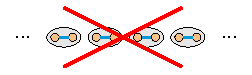
\includegraphics[width=\linewidth] {diagrams/trivial_chain_w_x.pdf}
				\vskip-0.4cm
				\caption{1D Trivial Chain}
			\end{figure}
			}
		\only<2>{
		\bi
		\item[] Product state with one boson per site
		\ei
		}
		\end{block}
	\end{column}
	\begin{column}[T]{.5\textwidth}
		\begin{block}{Topological Insulators}
			\vskip0.45cm
			\begin{figure}
				
\includegraphics[width=\linewidth] {diagrams/haldane_insulator_chain.pdf}
				\caption{1D Topological Chain}
			\end{figure}
		\only<2>{
		\bi
		\item[] Haldane Insulator Phase \cite{pollmann2010}
		\item Unitarily related to AKLT
		\item No $SU(2)$ symmetry
		\item Symmetry protected 2-fold edge degeneracy
		\ei
		}
		\end{block}
	\end{column}
\end{columns}
\only<1>{
\begin{center}
	\begin{figure}[]
		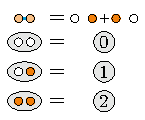
\includegraphics[width=0.4\textheight] {diagrams/haldane_insulator_chain_rules.pdf}
		\caption{Projectors and entangled pairs (PEPS) used in state construction}
	\end{figure}
\end{center}
}
\only<3>{
\begin{center}
	\begin{figure}[]
		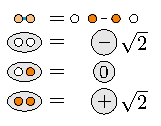
\includegraphics[width=0.4\textheight] {diagrams/aklt_rules.pdf}
		\caption{Projectors and entangled pairs (PEPS) for $SU(2)$ symmetric state}
	\end{figure}
\end{center}
}
\end{frame}

%Examples include free fermion band insulators, both trivial and topological
%Interacting 1D examples would include the spin-1 heisenberg AFM